\section{User interface design}
The goal of this section is to show the design of the main screens of the Customer-app and CPO-administration-app. 
It's described the flow of screens, according to the main functionalities for which the application was intended.

\subsection{Customer Mobile App}

\subsubsection{Sign-Up}
\begin{center}
    \begin{figure}[H]
        \includegraphics[width=\textwidth]{./img/design/app/Signup.png}
        \caption{Sign Up screens}
    \end{figure}
\end{center}
These mobile-app's sceens represent the graphical flow during the Sign-up procedure. Once user-data have been inserted and the continue button is pressed the mobile app sends a request to signUp to the eMSP. All the communication between the app and the eMSP use the eMSP's LoginInterface. After that the user is requested to press the confirmation link sent in the mail, and after a successful confirmation the user is redirected to the mobile-app's main page.

\subsubsection{Log-In}
\begin{center}
    \begin{figure}[H]
        \includegraphics[width=\textwidth]{./img/design/app/Login.png}
        \caption{Log-in screens}
    \end{figure}
\end{center}
These mobile-app's sceens represent the graphical flow during the Log-in procedure. The customer inserts his personal data and then presses Sign-in. This will call, using the eMSP's LoginInterface, the signIn methon on the application server.

\subsubsection{Stations view}
\begin{center}
    \begin{figure}[H]
        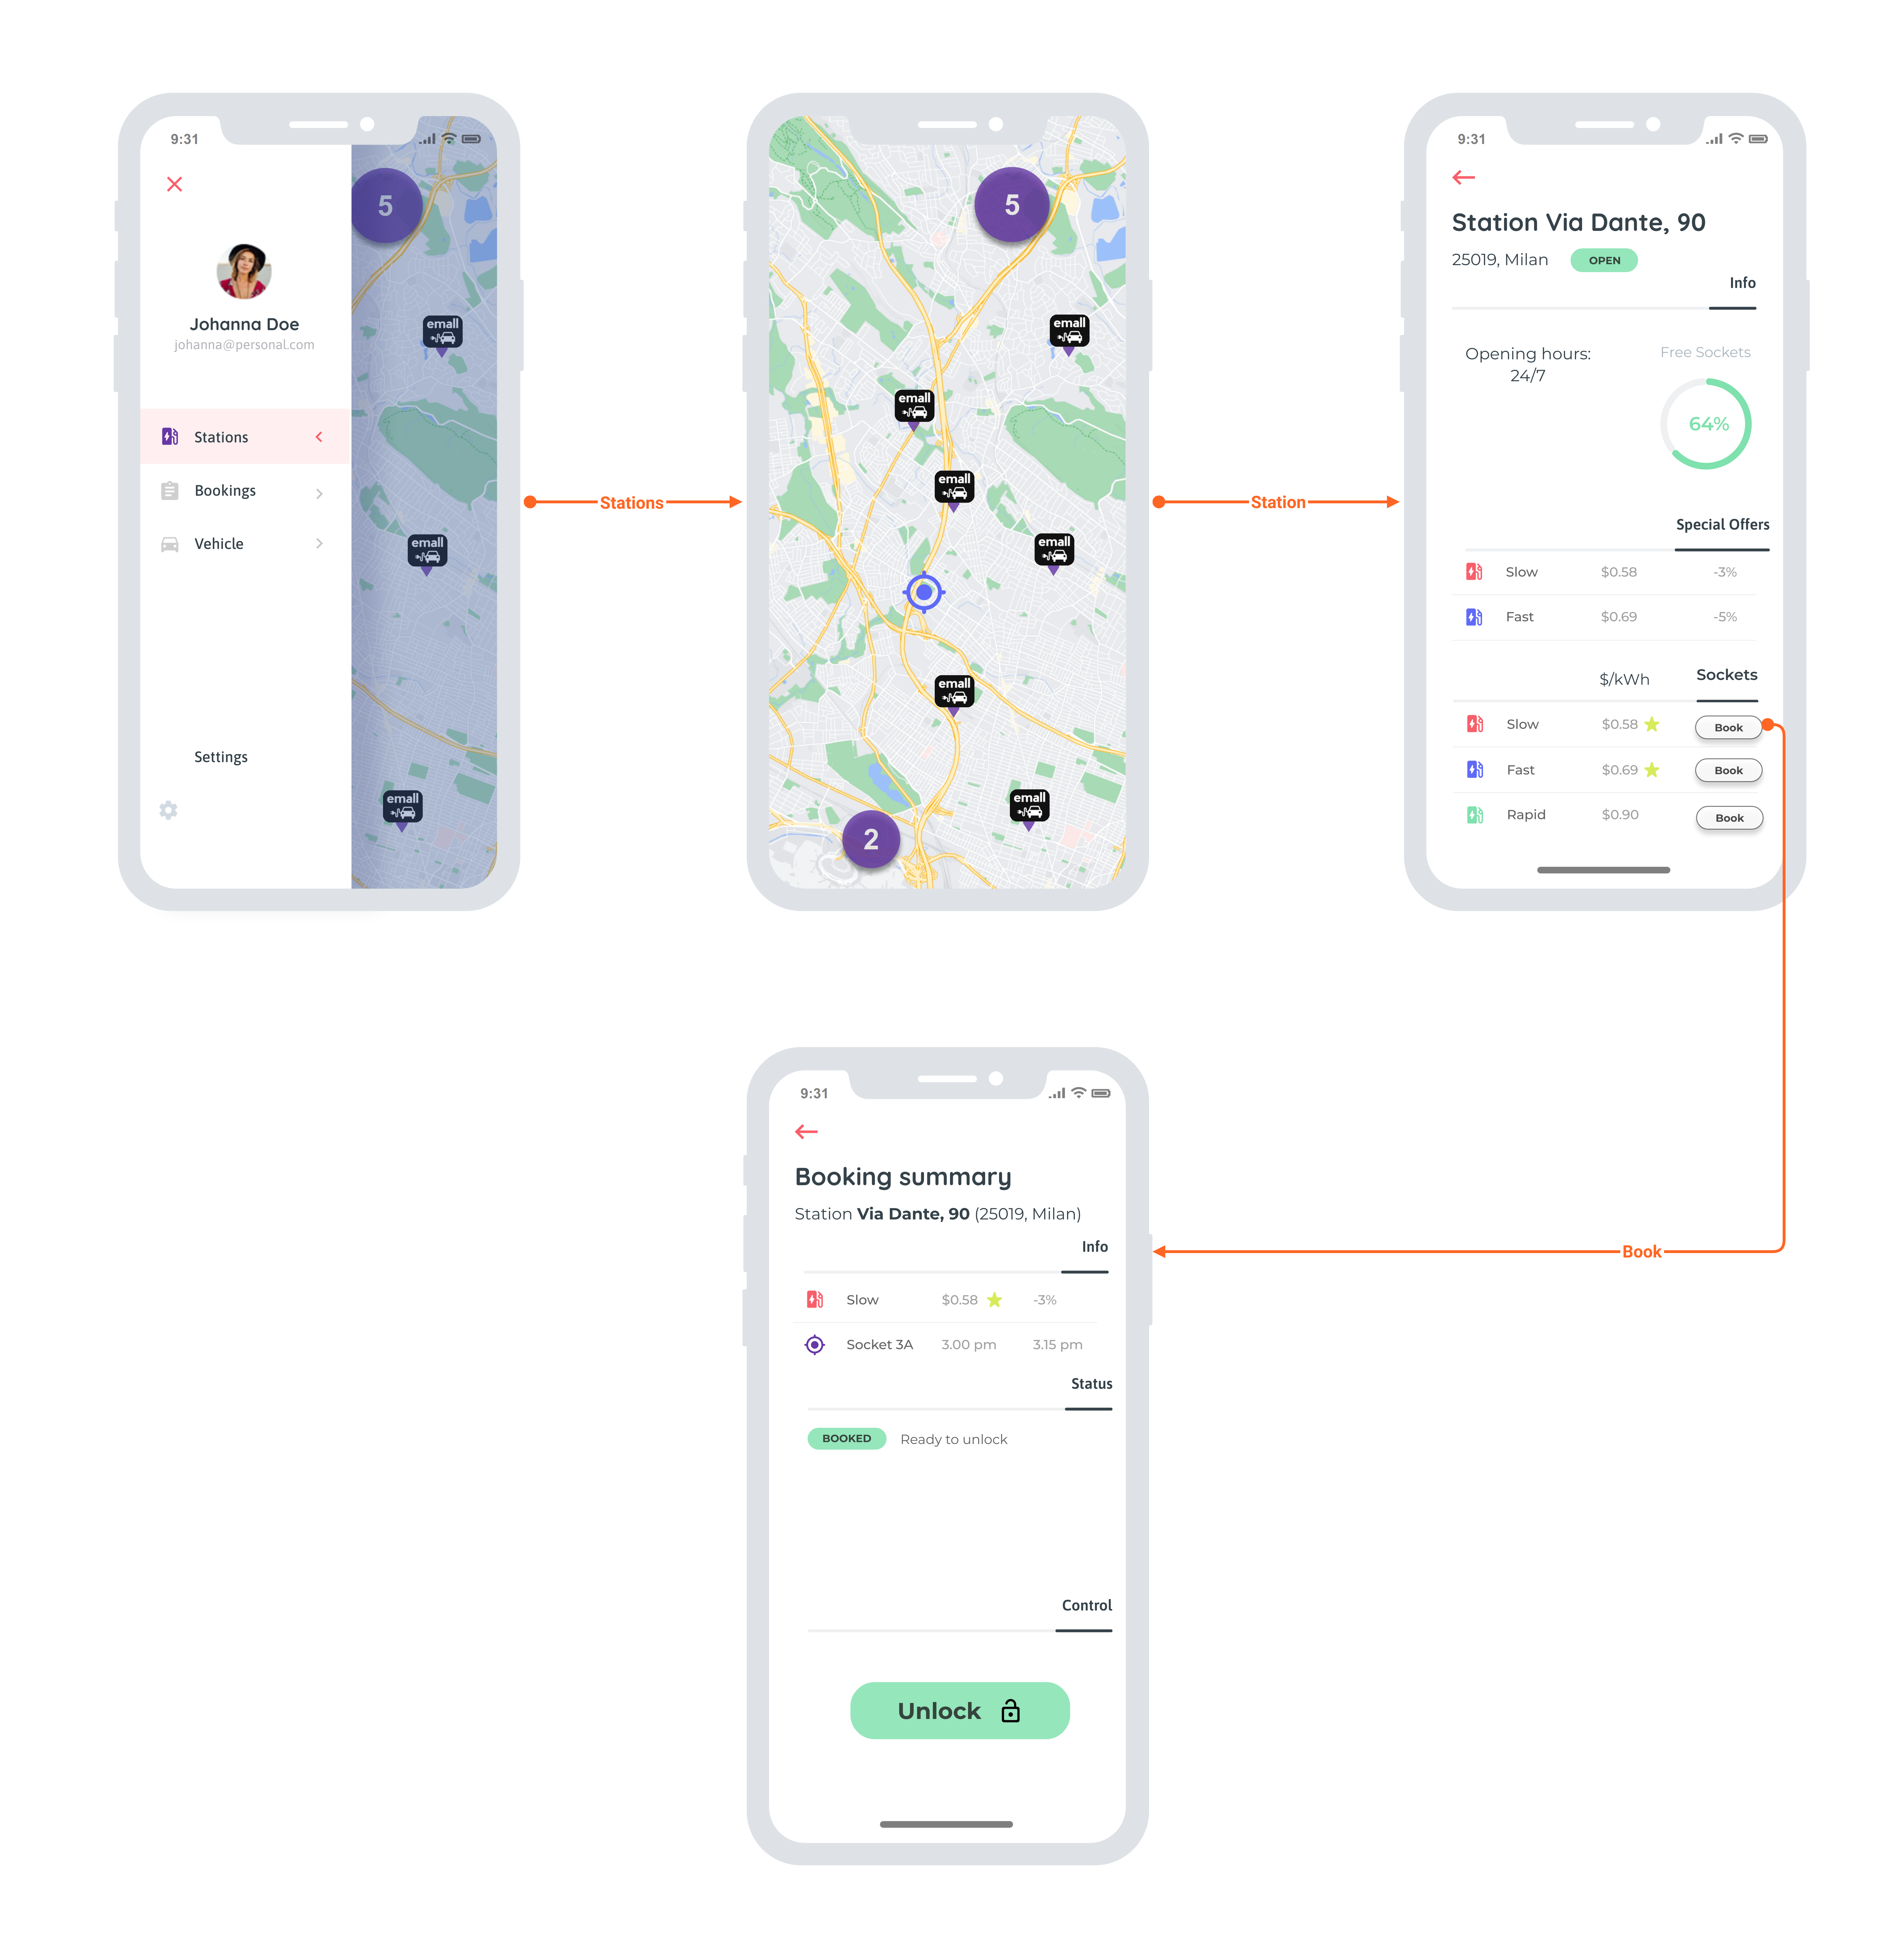
\includegraphics[width=\textwidth]{./img/design/app/Stations.png}
        \caption{View of the nearby stations and booking screen}
    \end{figure}
\end{center}
These mobile-app's sceens represent the graphical flow during stations searching. If the customer clicks on a station a request to the eMSP to get the station info is sent. If the user wants to book a charge he pushes the book button. The book button sends a request to the eMSP to book a socket.


\subsubsection{Bookings}
\begin{center}
    \begin{figure}[H]
        \includegraphics[width=\textwidth]{./img/design/app/Bookings.png}
        \caption{Booking screens}
    \end{figure}
\end{center}
Using the booking button the customer can see all his bookings (old and current booking). The customer clicking on a specific booking on the list can perform several actions. The customer can pay a booking. The customer can unlock the socket pushing the unlock button, after having unlocked the socket he is taken to the screen "connect to the socket". Finally he can push the start charge button. All the requests and responses from and to the eMSP and the mobile-app uses the eMSP's customerInterface.

\subsubsection{Vehicle}
\begin{center}
    \begin{figure}[H]
        \includegraphics[width=\textwidth]{./img/design/app/Vehicles.png}
        \caption{Vehicle change screens}
    \end{figure}
\end{center}
These mobile-app's sceens represent the graphical flow during the default vehicle change. If a user wants to change its vehicle, he must enter the new informations and click the button. All the requests and responses from and to the eMSP and the mobile-app uses the eMSP's customerInterface.

\subsubsection{Suggestion}
\begin{center}
    \begin{figure}[H]
        \includegraphics[width=\textwidth]{./img/design/app/Suggestion.png}
        \caption{Push notification, suggestion to charge your vehicle}
    \end{figure}
\end{center}
If the eMSP finds a suggestion, a push notification is sent to the app, suggesting to book a charge.



\subsection{CPO Administration Web-App}

\subsubsection{CPO login}
\begin{center}
    \begin{figure}[H]
        \includegraphics[width=\textwidth]{./img/design/web/login.png}
        \caption{CPO login screen}
    \end{figure}
\end{center}
With this screen the CPO can log in to the CPMS system. The requests and responses to retrive and set data use the CPMS's CPOLoginInterface

\subsubsection{Stations}
\begin{center}
    \begin{figure}[H]
        \includegraphics[width=\textwidth]{./img/design/web/home.png}
        \caption{Dashboard with a list CPO's stations}
    \end{figure}
\end{center}
This screen is a dashboard with all the stations of a CPO, basic information are shown. To edit the configuration (price, battery policy,...) of a specific station the CPO user have to press the Modify Button.  The requests and response to retrive and set data use the CPMS's CPOInterface

\subsubsection{Station-Dashboard}
\begin{center}
    \begin{figure}[H]
        \includegraphics[width=\textwidth]{./img/design/web/station.png}
        \caption{Dashboard to manage a single charging station}
    \end{figure}
\end{center}
This screen is a dashboard used to modify station specific parameters. It's made up of 4 blocks. Orange buttons are used to modify the settings, so for example to update the DSO provider, set special offers... Once an orange button is pressed a pop-up appears to modify the parameters. The requests and response to retrive and set data use the CPMS's CPOInterface